\subsection{Vague topology on the space of measures}

Let X be a locally compact space. On the space \(\mathcal{M}(\mathrm{X};\mathbf{C})\) , one can consider the topology of pointwise convergence in \(\mathcal{K}(\mathrm{X};\mathbf{C})\) , which we shall call the vague topology on \(\mathcal{M}(\mathrm{X};\mathbf{C})\) .

Since \(\mathcal{K}(\mathrm{X};\mathbf{C}) = \mathcal{K}(\mathrm{X};\mathbf{R}) + i\mathcal{K}(\mathrm{X};\mathbf{R})\) , the vague topology on \(\mathcal{M}(\mathrm{X};\mathbf{C})\) is defined by the semi-norms \(\sup_{1\leqslant i\leqslant n}|\mu (f_i)|\) , where \((f_i)_{1\leqslant i\leqslant n}\) is any finite sequence of functions in \(\mathcal{K}(\mathrm{X};\mathbf{R})\) (or in \(\mathcal{K}_{+}(\mathrm{X})\) ). To say that a filter \(\mathfrak{F}\) on \(\mathcal{M}(\mathrm{X};\mathbf{C})\) converges vaguely to a measure \(\mu_0\) signifies that

\[
\mu_ {0} (f) = \lim _ {\mu , \mathfrak {F}} \mu (f)
\]

for every function \(f \in \mathcal{K}(\mathrm{X};\mathbf{R})\) . For every function \(f \in \mathcal{K}(\mathrm{X};\mathbf{C})\) , the mapping \(\mu \mapsto \mu(f)\) is a vaguely continuous linear form on the space \(\mathcal{M}(\mathrm{X};\mathbf{C})\) .

PROPOSITION 13. --- Let X be a locally compact space and, for every \(x \in X\) , let \(\varepsilon_{x}\) be the Dirac measure at the point x. The mapping \(x \mapsto \varepsilon_{x}\) is a homeomorphism of X onto a subspace of the space \(\mathcal{M}(\mathrm{X};\mathbf{C})\) of measures on X, equipped with the vague topology. Moreover, if \(X'\) denotes the compact space obtained by adjoining to X a point at infinity \(\omega\) , then \(\varepsilon_{x}\) tends to 0 as x tends to \(\omega\) .

For every function \(f \in \mathcal{K}(\mathrm{X};\mathbf{C})\) , \(\langle f,\varepsilon_x\rangle = f(x)\) ; since \(f\) is continuous, this proves that the mapping \(x \mapsto \varepsilon_x\) is continuous. If \(x,y\) are two distinct points of \(\mathbf{X}\) , there exists a function \(f \in \mathcal{K}(\mathrm{X};\mathbf{C})\) such that \(f(x) = 1\) , \(f(y) = 0\) (No.~2, Lemma 1), which proves that \(\varepsilon_x \neq \varepsilon_y\) ; the mapping \(x \mapsto \varepsilon_x\) is therefore injective. Moreover, for every function \(f \in \mathcal{K}(\mathrm{X};\mathbf{C})\) , \(\langle f,\varepsilon_x\rangle\) tends to 0 by definition as \(x\) tends to \(\omega\) , therefore \(x \mapsto \varepsilon_x\) may be extended by continuity to \(X' = X \cup \{\omega\}\) by assigning to it the value 0 at the point \(\omega\) . This extended mapping is also injective, since \(\varepsilon_x \neq 0\) for all \(x \in X\) . It is therefore a homeomorphism of the compact space \(X'\) onto a subspace of \(\mathcal{M}(\mathrm{X};\mathbf{C})\) , since \(\mathcal{M}(\mathrm{X};\mathbf{C})\) is Hausdorff for the vague topology (GT, I, §9, No.~4, Cor. 2 of Th. 2).

PROPOSITION 14. --- In the space \(\mathcal{M}(\mathrm{X};\mathbf{C})\) of measures on a locally compact space \(\mathbf{X}\) , the cone \(\mathcal{M}_{+}(\mathbf{X})\) of positive measures is complete for the uniform structure deduced from the vague topology (hence is vaguely closed in \(\mathcal{M}(\mathrm{X};\mathbf{C})\) ).

For, consider a Cauchy filter \(\Phi\) for the vague uniform structure on \(\mathcal{M}_{+}(\mathrm{X})\) ; by definition, \(\mu_{0}(f) = \lim_{\mu,\Phi} \mu(f)\) exists for every function \(f \in \mathcal{K}(\mathrm{X}; \mathbf{C})\) and, by the principle of extension of inequalities, \(\mu_{0}(f) \geqslant 0\) for every function \(f \in \mathcal{K}_{+}(\mathrm{X})\) ; it follows that \(\mu_{0}\) is a positive measure on X (No.~5, Th. 1).

\pandocbounded{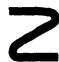
\includegraphics[keepaspectratio]{images/part001_58cd264b.jpg}}

It should be noted that the space \(\mathcal{M}(\mathrm{X};\mathbf{C})\) (or \(\mathcal{M}(\mathrm{X};\mathbf{R})\) ) itself is not necessarily complete for the vague uniform structure (TVS, II, §6, No.~7).

COROLLARY. --- If A and B are two vaguely closed subsets of \(\mathcal{M}_{+}(\mathrm{X})\) , then \(A + B\) is vaguely closed in \(\mathcal{M}_{+}(\mathrm{X})\) (hence also in \(\mathcal{M}(\mathrm{X};\mathbf{C})\) ).

This is in fact a general property of weakly complete, proper cones in locally convex spaces (TVS, II, §6, No.~8, Cor. 2 of Prop. 11).

PROPOSITION 15. --- Let H be a subset of \(\mathcal{M}(\mathrm{X};\mathbf{C})\) . The following properties are equivalent:

\begin{enumerate}
\def\labelenumi{\alph{enumi})}
\item
  H is vaguely bounded.
\item
  H is vaguely relatively compact.
\item
  H is equicontinuous.
\item
  For every compact subset K of X, there exists a number \(M_{K} \geqslant 0\) such that \(|\mu(f)| \leqslant M_{K}\|f\|\) for every measure \(\mu \in H\) and every function \(f \in \mathcal{K}(X, K; \mathbf{C})\) .
\end{enumerate}

Since \(\mathcal{K}(\mathrm{X};\mathbf{C})\) is a barreled space (No.~1, Prop. 2), the equivalence of properties a), b) and c) follows from TVS, III, §4, No.~1, Scholium.

It is clear that d) implies a). Finally, if H is equicontinuous then the set of restrictions of the measures \(\mu\in H\) to \(\mathcal{K}(X,K;\mathbf{C})\) is also equicontinuous, whence the condition d), since \(\mathcal{K}(X,K;\mathbf{C})\) is a normed space.

* We shall see in Ch. IV, §4, No.~6 that the conditions of Proposition 15 are also equivalent to the condition that, for every compact subset K of X, there exists a constant \(\mathrm{M}_{\mathrm{K}}\) such that \(|\mu|(\mathrm{K}) \leqslant \mathrm{M}_{\mathrm{K}}\) for every measure \(\mu \in \mathrm{H}\) .

COROLLARY 1. --- Let \(\nu\) be a positive measure on X; the set of measures \(\mu\) such that \(|\mu| \leqslant \nu\) is vaguely compact.

COROLLARY 2. --- The set of measures \(\mu\) such that \(\|\mu\| \leqslant a\) (a any finite number \(>0\) ) is vaguely compact.

COROLLARY 3. --- If X is compact, the set of positive measures \(\mu\) on X such that \(\|\mu\| = 1\) is vaguely compact.

For, it is the intersection of the vaguely compact set (Cor. 2) of measures such that \(\|\mu\|\leqslant1\) and the vaguely closed sets defined respectively by the relations \(\mu\geqslant0\) and \(\mu(1)=1\) (No.~8, Cor. 2 of Prop. 10).

COROLLARY 4. --- In the space \(\mathcal{M}(\mathrm{X};\mathbf{C})\) , the mapping \(\mu \mapsto \| \mu \|\) is lower semi-continuous for the vague topology.

This is an immediate consequence of Corollary 2.

\pandocbounded{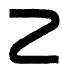
\includegraphics[keepaspectratio]{images/part001_13b41992.jpg}}

It should be noted that the mapping \(\mu \mapsto |\mu|\) of \(\mathcal{M}(\mathrm{X};\mathbf{C})\) into itself is not necessarily continuous for the vague topology (Exer. 9).

PROPOSITION 16. --- Let K be a compact subset of X, H a vaguely bounded subset of \(\mathcal{M}(\mathrm{X};\mathbf{C})\) ; then, the bilinear form \((f,\mu)\mapsto\langle f,\mu\rangle\) is continuous on \(\mathcal{K}(\mathrm{X},\mathrm{K};\mathbf{C})\times\mathrm{H}\) when \(\mathcal{K}(\mathrm{X},\mathrm{K};\mathbf{C})\) is equipped with the topology of uniform convergence and H with the vague topology.

For, there exists a number \(M \geqslant 0\) such that

\[
| \mu (f) | \leqslant \mathrm{M} \| f \|
\]

for every function \(f \in \mathcal{K}(\mathrm{X},\mathrm{K};\mathbf{C})\) and every measure \(\mu \in \mathrm{H}\) (Prop. 15). If \(\mu_0\) and \(\mu\) are two measures belonging to \(\mathrm{H}\) , \(f_0\) and \(f\) two functions in \(\mathcal{K}(\mathrm{X},\mathrm{K};\mathbf{C})\) , then

\[
\begin{array}{r l} | \mu (f) - \mu_ {0} (f _ {0}) | & = | \mu (f - f _ {0}) + \mu (f _ {0}) - \mu_ {0} (f _ {0}) | \\ & \leqslant \mathrm{M} \| f - f _ {0} \| + | \mu (f _ {0}) - \mu_ {0} (f _ {0}) |, \end{array}
\]

and the last quantity is arbitrarily small when \(\|f-f_{0}\|\) and \(|\mu(f_{0})-\mu_{0}(f_{0})|\) are, which proves the proposition.
% semantic-fragments: legacy-input-seam
\relax{}
